\section{Results}
  % Here the results of our study, within the bounds of our study only, should be discussed - times, most effective distributions, potential reasoning as to why.
  % The next section handles the relation of this to the real world.
\subsection{Control Results}

\subsection{Main Results}

\begin{figure}[H]
  \centering
  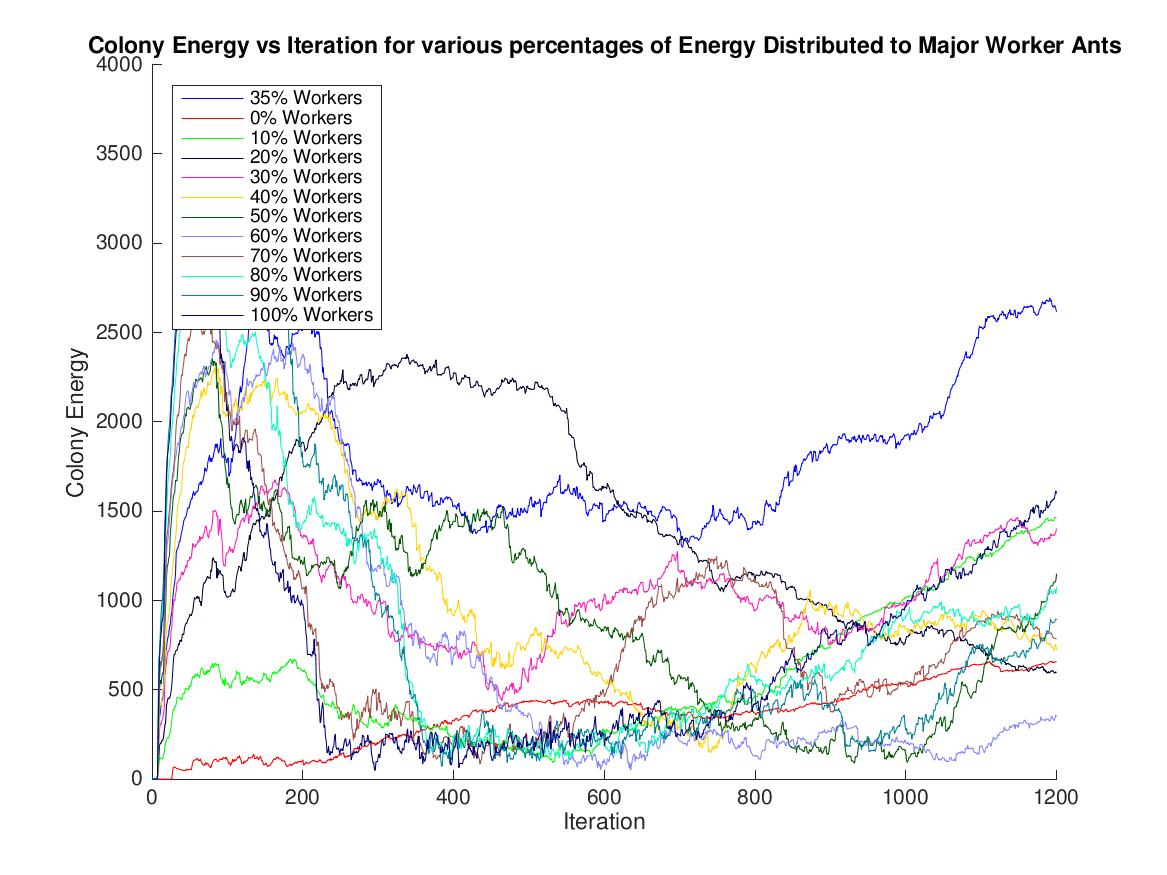
\includegraphics[width=1\textwidth]{images/line-graph-results.png}
  \caption{Line graph depicting colony energy against iterations (time) for various percentages of Major Worker Ant.}
  \label{fig:iters-line}
\end{figure}

\begin{figure}[H]
  \centering
  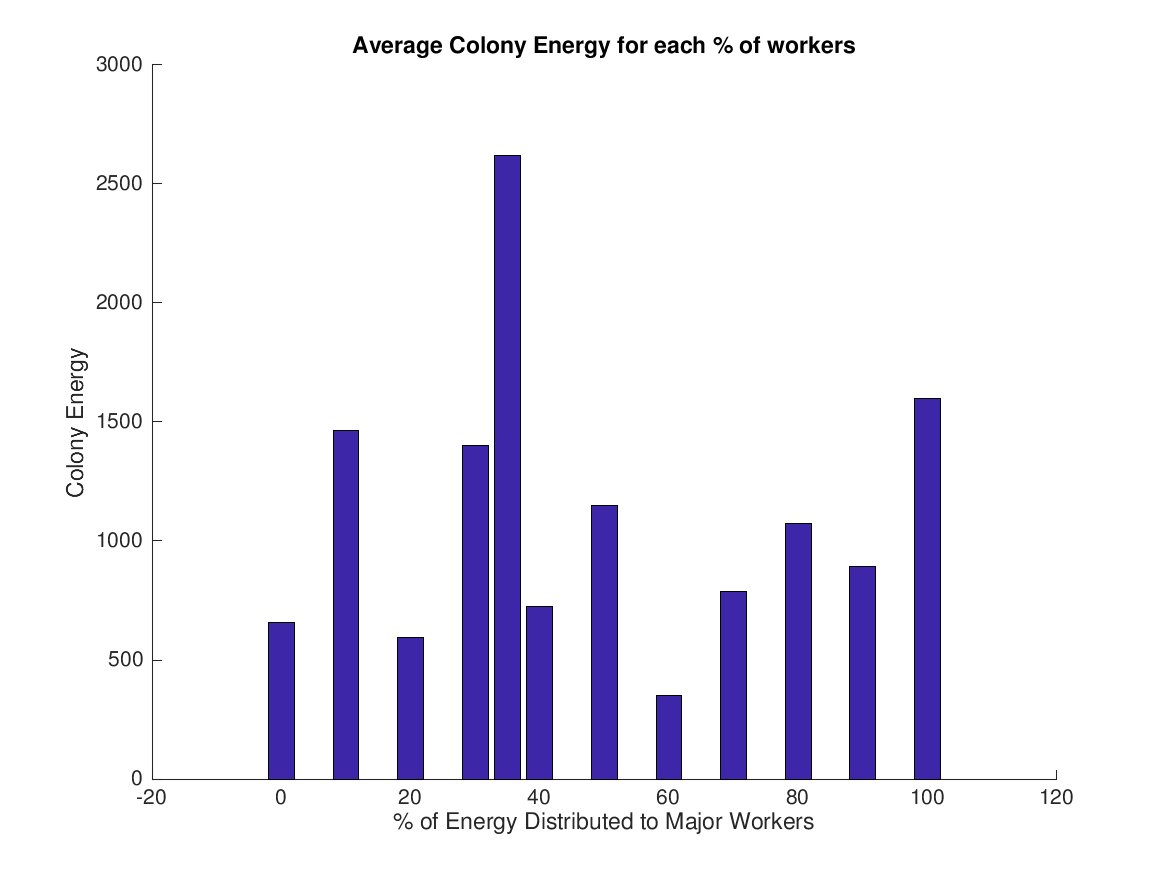
\includegraphics[width=1\textwidth]{images/bar-chart-results.png}
  \caption{Bar Chart depicting colony energy against iterations (time) for various percentages of Major Worker Ant.}
  \label{fig:iters-bar}
\end{figure}

\subsection{Repeatability}
